\documentclass[11pt,twoside,a4paper]{article}
\usepackage[english]{babel}
\usepackage{amsmath}
\usepackage{amsthm}
\usepackage{amssymb}

\usepackage[pdfstartview=FitH,pdfpagemode=UseNone]{hyperref}
\usepackage[letterspace=40]{microtype}

\usepackage{a4wide,times}
\usepackage{graphicx}
\usepackage{color}
\usepackage[section]{placeins}

\urlstyle{same}
\linespread{1.1}

\title{
  IN4086 Data Visualization\\
  Final Project\\
  ``Teamfight Classification and Visualization in\\ Defense of the Ancients 2 (DotA2)''
}
\author{
    Tung Phan, ttphan, 4004868 \and
    Kevin van Nes, kjmvannes, 4020871
}

\begin{document}

\maketitle
%For the final project we would like to expand our work on classifying and visualizing teamfights and their corresponding information. This work was started as part of Assignment 1 for this course. We were very excited about the assignment and we think it would be very interesting to see whether we could visualize other information with respect to teamfights.
%The tools we will use to reach this goal are the same ones we used for the first assignment: D3 and Javascript. We found that working with D3 helped a lot when it came to reading the data and visualizing it properly.
%We can not yet concretely define our deliverables. We want to do research into what kind of improvements can still be made to the existing results that we obtained from the first assignment. A general approach that we want to take is to visualize the data in such a way that both skilled and unskilled players can quickly retrieve information about the most interesting parts of a match. We had been thinking of adjustments such as being able to `slide' through a game and see teamfight locations (and possibly other things, such as objective control) throughout the game. We also want to create a way in which players can view and compare the teamfights of multiple matches at the same time. Lastly, if time allows it, we want to try and see if we can come up with interesting features and visualizations that do not directly involve teamfights. One thing we came up with was the visualization of objective control (killing creeps in the jungle, fighting near towers, etc.).
%We hope to see some more interesting results while working on this project!
\newpage
\section*{Introduction}
%Talk about how part of the application was already created and that we really wanted to improve the application in terms of visualization and the thereby given information.
The following report will discuss the application that was created as part of the final assignment of the IN4086 Data Visualization course. In this report we will explain why this application was created and its functionalities in terms of visualization and providing information to the user will be elaborated upon.
\newline\newline
The main role of the application is to extract so-called `teamfights' out of data from the Multiplayer Online Battle Arena game called `Defense of the Ancients 2' or DotA2. The goal is to extract and visualize these teamfights and to give users information about these teamfights in many different, but clear ways.
\newline\newline
Preliminary work for this application was done during the first assignment for the Data Visualization course. As a result of this assignment, we had gone through the Data Processing steps, with which we were able to set up a basic application which itself provided a basic visualization of the data and corresponding information. The process behind this preliminary work will be described later on in this report.
\newline\newline
Our goals for this project were to improve the ways in which information was visualized and provided to the users of the application. We wanted to improve the application so that it would visualize the match data in such a way that both skilled and unskilled players are able to retrieve the information they seek to find. We also found it important to improve the amount of information that was provided with the given visualization and we wanted to create more extensive visualization and options for users, instead of just having the map of the DotA2 arena.
\newline\newline
The outline of the report is as follows. Firstly, in section \ref{sec:dataproc} (``Data Processing'' ), we will give a definition of how we interpreted teamfights. This will be done to avoid ambiguities in understanding our application and the rest of the report. Furthermore, we will describe what the application looked like and what it could do prior to the work that was done as part of the final assignment. After that, in  section \ref{sec:mov} (``Manners of Visualization'' ), the additions and improvements that were made to the application will be expanded upon. Finally, a short conclusion will be given in section \ref{sec:endresult}, in which we will discuss whether all goals were reached and what future work is planned to further improve the application.

\section{Data Processing}
\label{sec:dataproc}
%Talk about how we tried to follow the Data Visualization pipeline as much as possible, except for the Data Acquisition part, because data was already given.
The data visualization pipeline was followed during the preliminary work that was done as part of the first assignment. While improving the application for the final project, this pipeline was reiterated and improvements were made wherever we thought it was necessary or desirable. Of course, the Data Acquisition part of the pipeline was already done for us, as the files containing the match data were handed to us prior to making the assignment. We will firstly define how we used the word `teamfight' while creating the application. Furthermore, each of the steps of the data visualization pipeline (filtering, mapping and rendering) and their applications to our product will be discussed.

\subsection{Our Definition of Teamfight}
%Definition of teamfight for this application, just to make it clear to the reader and to avoid ambiguities.
To make sure that it is clear how we defined `teamfight' while designing and developing our application, we will define this in the upcoming paragraph. Teamfights are critical to the game, because a teamfight with all members involved are events with very high stakes. When one team has more team members alive than the other team as a result of that team fight, they can use this to their advantage by completing objectives or even finishing the game, while the dead members of the team who have lost the teamfight will have to either buy themselves in with their hard earned gold or wait for the respawn timer. Completing objectives will yield gold and territorial advantages to the winning team, which will cause a snowball effect throughout the game. In other words, teamfights involving all members of both teams determine the flow of the game.
\newline\newline
We define a teamfight as a period of time in which all players of both teams (Team Radiant and Team Dire) are close to their teammates and their enemies. Simply stated, this means that all ten players are near each other, which means that the chances of them fighting each other is very likely. This makes the period of time during which this happens a teamfight. We limit the teamfights to balanced teamfights of full capacity, balanced because it is a fight of even numbers and full capacity because all 10 players are involved. The moment one member is either killed or has retreated, the advantage is to the other team and we will not consider it a balanced teamfight of full capacity anymore. That also means that small skirmishes of less than 10 people are not considered teamfights, even if they are evenly balanced. This is to ensure that we only capture the teamfights where both teams go `all in'.

\subsection{Data Filtering}
%Describe the steps taken to extract teamfights
As was stated in the previous paragraph, a teamfight is a period of time during which all players in the game are fighting. We had come up with a way to extract these moments from the raw data files. Firstly, we wrote a simple script in Java that cut up the `master-distance.csv' and `master-zones.csv' files into separate files for each match (e.g. match-\textless match number\textgreater-distance.csv and match-\textless match number\textgreater-zones.csv). We were now able to extract the necessary variables to find teamfights out of each match.
\newline\newline
From the -zones files, we used the following variables: the x and y positions, the team the player belongs to, which team won and lost (WinLose) and the tsync variable (the current match time). From the -distance files, we used the same variables with the addition of the `DD' variable. The `DD' variable estimates the distance between members of each team, so for Team Dire, this variable calculates the distance between the five members of Team Dire, and vice versa for Team Radiant.
\newline\newline
For each match, we calculated for each tsync (= second) whether the DD variable was lower than a certain threshold. If it was, that time moment was added to an array along with its corresponding DD. We did this for both teams, resulting in two arrays containing low DD time moments for the winning team and the losing team, which we called winSmallDDArray and loseSmallDDArray, respectively. By intersecting these arrays, the smallDDArray was created, in which moments in time are contained where the DD is low for both teams at the same time. Such a moment means that players from both teams are close to their teammates. The only thing that remains to have a teamfight, is that both teams have to be close to each other at such a moment.
\newline\newline
To calculate whether this is the fact, we also calculated for each entry of smallDDArray the x and y positions of each of the ten players, so we also knew where a teamfight took place on top of when it took place. These positions were put into corresponding arrays too, which were again split up into a `winning team' and `losing team' version. Out of these positions, we were able to calculate the average positions of each team (i.e. the positions of all five players of a team, summed up and then averaged), with which we were now able to compute the Euclidean distance between these two averages. If this distance is lower than a certain threshold (we set this to 30, as we calculated this was a reasonable distance), a teamfight is found.
\newline\newline
With the above described procedure, we were able to find teamfights very accurately. We checked whether our estimations were right by downloading some of the replay videos corresponding to the match numbers and checking whether a teamfight actually took place during the timespans that we estimated and it turned out we were able to find teamfights really accurately. This meant that we could now start on mapping the data to renderable data.

\subsection{Data Mapping}
\label{subsec:datamapping}
%Talk about the clusters that we mapped each of the teamfights to, containing properties of a teamfight that we used to render the ellipses.
As was stated above, the teamfights that we were now able to find needed to be mapped to renderable data. For this purpose, we decided to put each teamfight in a corresponding cluster object, which contains useful properties of the corresponding teamfight. The most important properties for rendering the data were the average x and y positions and the lowest and highest x and y positions of the teamfight. The average x and y positions are simply calculated by summing all of the x and y positions of the teamfight and averaging them. The lowest and highest x and y positions were computed by taking the lowest/highest x/y position that was fought on.
\newline\newline
These values could be mapped to create ellipses, which visualize the area of a teamfight in a visually clear and computationally efficient way. The average x and y positions of the clusters (and thus the teamfights) are used to decide where the center points of the ellipses need to be drawn, while the lowest and highest x and y values of the teamfight are used to compute the x and y radiuses of the ellipses. These ellipses will - when rendered - visualize the main part of each teamfight of a match.
\newline\newline
Since teamfights are usually fought in areas that are not easily visualized by geometry, we had chosen to use ellipses, as these forms would give the most smooth results when visualizing a teamfight. If we had for example used a rectangle, the result would be too rough. We also experimented with a different kind of visualization (i.e. drawing small circles/dots for each position a teamfight had taken place in). This type of visualization was, even though it showed the area of teamfights more accurately, less optimal, as poor results were obtained in case a lot of teamfights were fought in a match. The user of the application would in these cases quickly lose the overview and the visualization would quickly become polluted and unclear, which is something we had avidly tried to avoid.

\subsection{Data Rendering}
\label{subsec:datarendering}
Now that we mapped the data to the ellipses, rendering was an easy step, as we used the D3 library \ref{ref:d3}
 to draw the ellipses easily using the computed variables and properties of the teamfights. The colors of the ellipses are determined using a combination of three qualitative contrasting color scales. These color scales are extracted from the ColorBrewer application \ref{ref:colorbrewer}.
These scales were used to make sure that all ellipses contrasted as much as possible so that the visualization is not unclear and does not contain ambiguities. 
The ellipses are also drawn with slight transparency, this is done to make sure that no invisible overlaps (i.e. one ellipse falls completely behind another) happen when two teamfights occur in the same area.
\newline\newline
To get an idea of what the application looked like after this preliminary work, see Figure~\ref{fig:oldapp}.

\begin{figure}[ht]
\centering
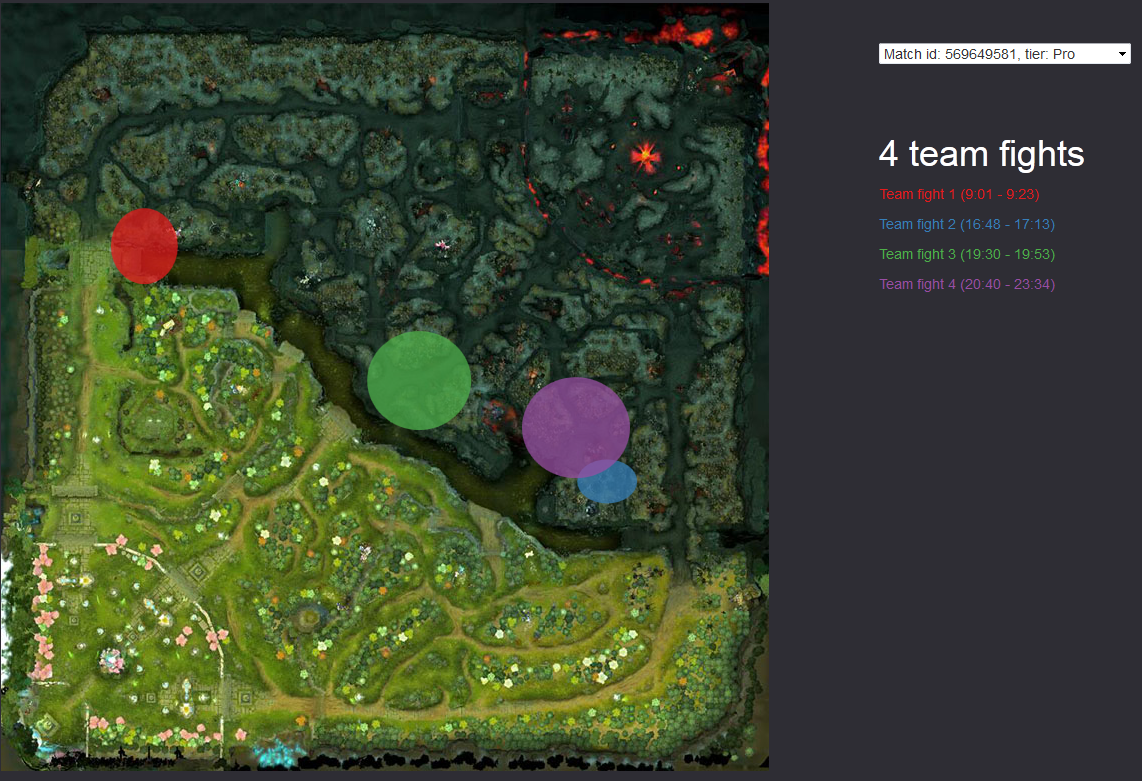
\includegraphics[width=\textwidth]{oldApp.png}
\caption{An overview of the old application}
\label{fig:oldapp}
\end{figure}

A new challenge arised when we decided to extend the application in such a way that the teamfights of two matches could be compared, instead of just showing the teamfights of one match. This meant that colors would have to be different for teamfights of different matches and that the shapes would have to differ too. More about this newly arised challenge will be discussed in section \ref{subsec:map}.

\section{Manners of Visualization}
\label{sec:mov}
%Short intro of the different tools for visualization and information. Tell something about the coherence between parts of the application.
The previous section described in detail how the application worked after the preliminary work. From this point on, we wanted to improve and extend the application as part of the Data Visualization final project. Our main goals were to extend the amount of visualization that is done by the application and to enlarge the amount of information that can be retrieved from the data for both skilled and unskilled DotA2 players. 
\newline
To keep the explanation as clear as possible, we have split up the application into three parts, which will be discussed separately below. Of course, any coherency will also be expanded upon. The three parts we have split up our application into are the following: the map, the menu and the timeline and brush.

\subsection{Map}
\label{subsec:map}
%Talk about the ellipses that are drawn on the map for each match, the different colors (qualitative contrasting) and shapes (fills) of the teamfight ellipses when comparing 2 matches, why not more than 2 matches (because each match would make the visualization less clear and this would be hard to solve in terms of different shapes/colors, etc. in our application) and last but not least: the tooltips, giving more information about each teamfight. Also if an ellipse is hovered over, the corresponding text in the sidebar on the right is enlarged, showing the user which teamfight he/she is highlighting, which brings more clarity.
The image in the upper left part of our application is called the map. This image represents a top-down view of the arena in which DotA2 matches are played. The map is also the part of our application where the ellipses representing the teamfights are drawn.
As can be seen in Figure \ref{fig:oldapp}, the application was merely able to show ellipses and their timespans for one match, without any additional information.
\newline\newline
Our first goal for enhancing this part of the application was to add the ability to compare two matches with each other, while still maintaining a clear visualization of the teamfights of both matches.\newline
After having created the menu to add two teamfights - which will be elaborated in section \ref{subsec:menu} - we needed to think about how to avoid causing confusion when visualizing the teamfights of two matches together. We wanted to use the same elliptic shapes to visualize teamfights of a second match (for the reasons described in section \ref{subsec:datamapping}), but differences had to be made to clearly visualize which ellipse belongs to which match. The first solution we applied to do so was to use different colors and textures for the ellipses of the second match compared to those of the first match. The ellipses of the second match were given colors from the end of the array containing the qualitative contrasting color scale, as to make sure that reoccurring colors are a rare occurrence. Furthermore, the second match ellipses are shown as the perimeters of an ellipse (so only an elliptic line), instead of a filled ellipse. This was chosen as a suitable solution, because the filled ellipses of one match contrast the elliptic lines of another very well. The colors are also set to be contrasting as much as possible, meaning that confusion will probably not occur very quickly. Furthermore, the elliptic lines will not hide (i.e. overlap) other teamfights, because one can see through the unfilled area in the middle.\newline\newline
Another goal we had, was to give users more information about each of the teamfights. This information was retrieved from the same data as was used to draw the ellipses. To give this information to the user in a clear fashion, we used the Tipsy library \ref{ref:tipsy}
to develop tooltips that appear whenever a user hovers over one of the ellipses. These tooltips contain information about the main areas the teamfight was fought in and about its duration. Whenever a user hovers over an ellipse, the other ellipses are turned gray and the text in the menu on the right corresponding to the ellipse is enlarged. This is done to emphasize to the user which teamfight he/she is looking at, so he/she can for example decide to hide this ellipse from the view.\newline\newline
More emphasis on the connection between ellipses and the menu on the right is made due to the fact that the colors of the ellipses of both matches correspond to the colors used to color the texts in the menu on the right. The colors are also connected to those of the rectangles shown on the timeline, which is discussed in section \ref{subsec:timeline}.
\newpage
\subsection{Menu}
\label{subsec:menu}
%Talk about menu and why it was added to the application. Allows for very specific kinds of visualization of matches, e.g. comparing 2 matches, but also checking/unchecking certain teamfights because a person might want to see all teamfights that happened in a certain area of the map or someone might want to compare the first teamfight that happened in each match.
Since we want to offer users of the application as much freedom of choice as possible when it comes to what and how they want to visualize teamfights, we have enhanced the menu to the right of the map as a part of reaching this goal. As was discussed in the previous section, we have added a second dropdown menu to allow users to compare the teamfights of two different matches. We understood that users might not want to scroll through the whole list of matches every time they are looking for a match of a specific tier. Therefore, we have made it possible to filter matches by player skill tier, making it easier for users to make specific comparisons, e.g. comparing two pro matches, or a pro and a normal match.
\newline\newline
Furthermore, we made sure to stay consistent with the visualization that happens on the map, which means that we also added the functionality of tooltips appearing when a user hovers over one of the teamfight texts. The ellipse corresponding to the text that is hovered over in the menu will be highlighted on the map.

\subsection{Timeline and Brush}
\label{subsec:timeline}
%Talk about timeline and brush and the added value of both of these (timeline -> relative positions in time of teamfights in a match,    brush -> easier filtering than clicking all of the select boxes separately, which also allows for new visualization options, e.g. seeing all teamfights that happened after the 15th minute)
One of the last goals we had stated in our project proposal was the addition of the possibility to `slide' through games. We wanted to add this to the application to give users even more options for visualizing teamfights. To this end, we have implemented a timeline with a `brush', which are also often used in parallel coordinate plots.\newline
The timeline can be found below the map. On the timeline small rectangles are placed, which represent the teamfights and their durations. A longer rectangle represents a longer teamfight. The colors of these rectangles also correspond to those of the ellipses and menu texts. The timeline also visualizes the relative positions and lengths of teamfights of one or both matches. Furthermore, the white vertical line, which is shown on the timeline as soon as two matches are compared, represents the end of the shortest of the two matches.\newline\newline
The addition of the brush to the timeline gives users the ability to `slide' through a game and filter specific moments of the game. This gives the users new visualization options, such as for example being able to see all teamfights that happened after the first fifteen minutes of a match have passed. 

\section{End Result}
\label{sec:endresult}
%Show end result, maybe talk a bit about it?
An overview of what the application now looks like can be seen in Figure \ref{fig:endresult}. Below, we will review our goals, discuss in what ways we want to work further on our application to improve it in the future and give a short conclusion.

\begin{figure}
\centering
  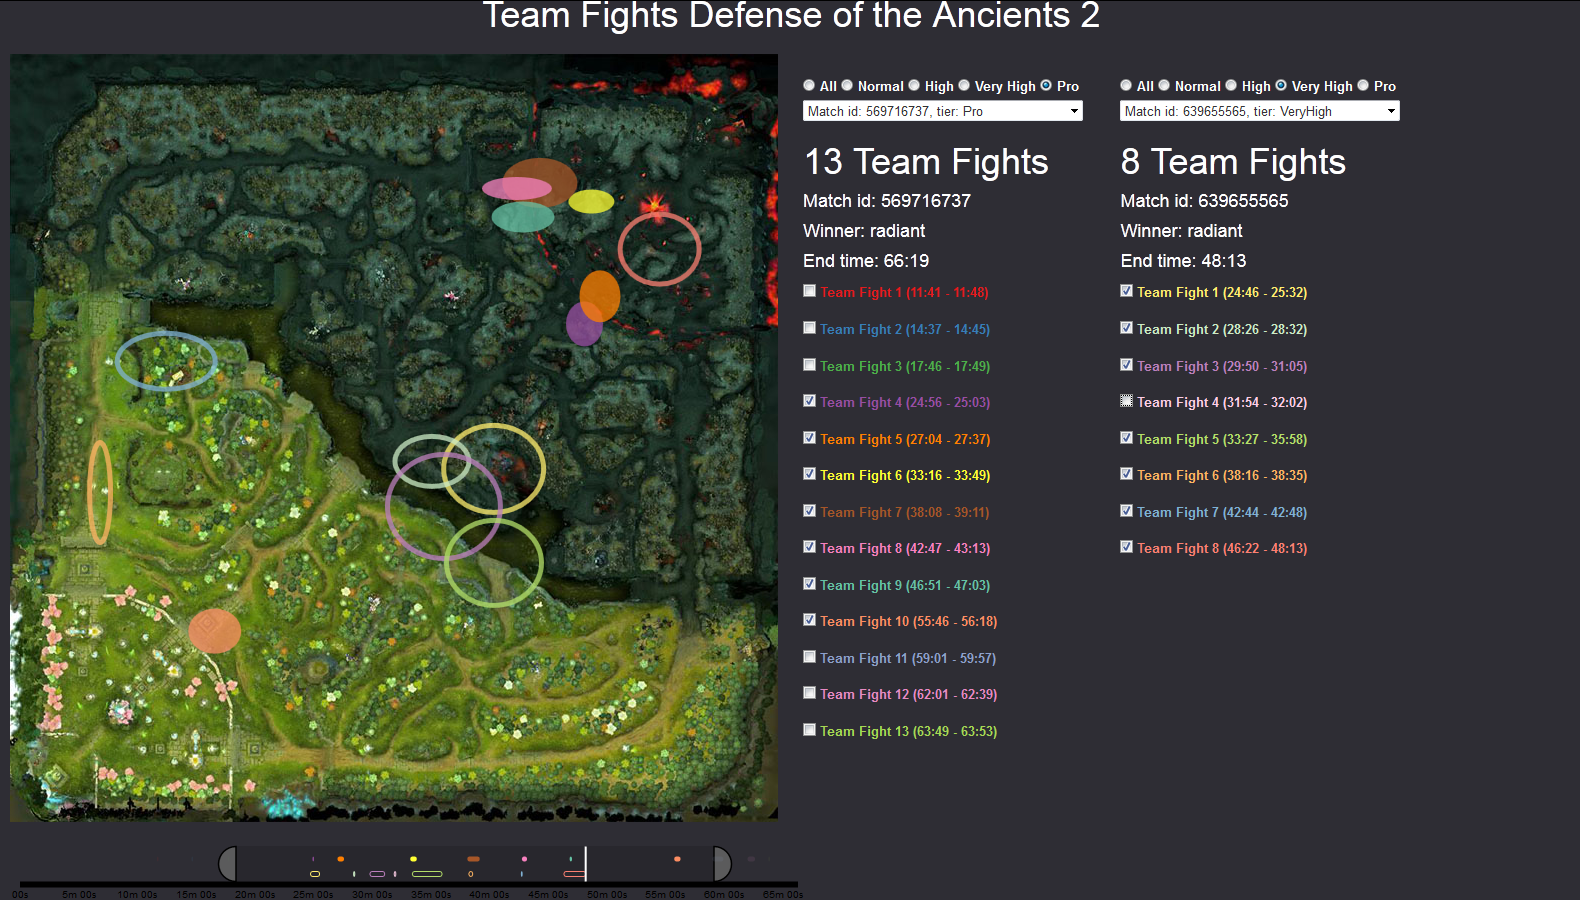
\includegraphics[width=\textwidth]{endResult.png}
\caption{The end result of our work: the application in its current state}
\label{fig:endresult}
\end{figure}

\subsection{Goals Review}
%We can not yet concretely define our deliverables. We want to do research into what kind of improvements can still be made to the existing results that we obtained from the first assignment. A general approach that we want to take is to visualize the data in such a way that both skilled and unskilled players can quickly retrieve information about the most interesting parts of a match. We had been thinking of adjustments such as being able to `slide' through a game and see teamfight locations (and possibly other things, such as objective control) throughout the game. We also want to create a way in which players can view and compare the teamfights of multiple matches at the same time. Lastly, if time allows it, we want to try and see if we can come up with interesting features and visualizations that do not directly involve teamfights. One thing we came up with was the visualization of objective control (killing creeps in the jungle, fighting near towers, etc.).
We have reached most of our goals during this project. Our first goal was to make sure that both skilled and unskilled players can quickly retrieve information about the most interesting parts of a match, e.g. teamfights. We have done our best to offer a lot of possibilities and options that help the user, either skilled/unskilled, to visualize exactly what he/she wants to find out.\newline
Another goal of ours was to add the ability to `slide' through games. The addition of our timeline and brush has made this possible, which opened up a lot of new ways to visualize specific information about teamfights, such as their relative position to each other.
\newline
A goal that was constantly kept in mind was that all of our work should adhere to the principles of Data Visualization, which were taught to us during the course lectures. We have done our best to do this, so that our end result would become as good and clear as possible.
\newline\newline
Lastly, a goal that was not fulfilled was the addition of visualization of other DotA2 information. In our proposal we stated that, if time allowed it, we would try and see if we could visualize other interesting features of DotA2 matches, such as fighting near towers or killing jungle creeps. We had taken time to think about how we would do this, but we found out that it would be very hard to accurately visualize these things using only the data that was given to us. More information would have needed to be available.
However, we have enjoyed working on this application and visualizing this data very much, so we have decided to continue working on the application after this project has ended. We will talk about this in the next section.

\subsection{Future Work}
As stated above, we are still very enthusiastic about data visualization and also about its relation with game data in this case. We want to see if there are ways to get more information out of matches, so that we will still be able to visualize such things as were mentioned above (fighting near towers, killing jungle creeps, etc.).\newline
Some of our more ambitious ideas include adding the option to include the replay videos of matches within the application. We would then give users the possibility of clicking a teamfight ellipse, which would then bring the replay video to the point in time where that specific teamfight started. This way, users will be able to watch specific teamfights without having to remember at which times these teamfights took place. They could simply look them up!

\subsection{Conclusion}
We are happy with the end result of our work. The application does what we wanted it to do and it does this in a smooth and clear way. We think it also conforms to the principles of Data Visualization as they were taught to us during the course lectures.
The end result of our application can be found on \url{http://www.techteach.nl/dota2}

\newcounter{refcounter}

\section{References}
Bostock, M. (2013). Data-Driven Documents (Version 3.5.4) [Software]. Available from http://d3js.org/ \refstepcounter{refcounter}\label{ref:d3}
\newline
Brewer, C., \& Harrower, M. ColorBrewer (Version 2.0) [Software]. Available from http://www.colorbrewer2.org/ \refstepcounter{refcounter}\label{ref:colorbrewer}
\newline
Frame, J. (2012). tipsy (Version 1.0.0a) [Software]. Available from http://onehackoranother.com/projects/jquery/tipsy/ \refstepcounter{refcounter}\label{ref:tipsy}

\end{document}